\documentclass[../Article_Model_Parameters.tex]{subfiles}
\graphicspath{{\subfix{../Figures/}}}
\begin{document}
		
	For the sake of clarity of the process model, different colors have been used in the equations to indicate: 
	{\color{red}control variables},
	{\color{blue}state variables},
	{\color{orange}variables} and
	{\color{magenta}parameters}.
	
	\subsubsection{Continuity equation} \label{CH: Continuity}
	The continuity equation for the fluid phase is derived in Appendix \ref{CH: Gouverning equations}. When the cross-sectional area of the channel $A_f$ is specified as a function of the void fraction ${\color{magenta}\phi}(z)$ (where ${\color{magenta}\phi}$ is the void fraction of the bed and $A$ is the cross-section of the empty extractor), the continuity equation takes the form: \todo[]{assign color to v and u}
	
	{\footnotesize
		\begin{equation*}
			\frac{\partial ({\color{orange}\rho_f}({\color{blue}T}(t,z),{\color{red}P}(t)) {\color{magenta}\phi})}{\partial t} + \frac{\partial ({\color{orange}\rho_f}({\color{blue}T}(t,z),{\color{red}P}(t)) v A {\color{magenta}\phi})}{\partial {\color{blue}z}} = 0
		\end{equation*}
	}
	
	Assuming that the mass flow rate is constant in time, the temporal derivative becomes zero, and the spatial derivative can be integrated along ${\color{blue}z}$ as
	
	{\footnotesize
		\begin{equation}
			\int \frac{\partial ({\color{orange}\rho_f}({\color{blue}T}(t,z),{\color{red}P}(t)) v A {\color{magenta}\phi})}{\partial {\color{blue}z}} dz = 0 \rightarrow {\color{red}F}={\color{orange}\rho_f}({\color{blue}T}(t,z),{\color{red}P}(t)) v A {\color{magenta}\phi}
		\end{equation}
	}
	
	Here, ${\color{red}F}$ is a constant obtained from the integration and is understood as the mass flux per unit area, which is assumed to be constant along ${\color{blue}z}$. To simplify the dynamics of the system, it is assumed that ${\color{red}F}={\color{red}F}(t)$ is a control variable and affects the whole system instantaneously. This assumption allows for finding the velocity profile that satisfies mass continuity based on ${\color{red}F}(t)$, ${\color{magenta}\phi}(z)$, and ${\color{orange}\rho_f}({\color{blue}T}(t,z),{\color{red}P}(t))$.
	
	{\footnotesize
	\begin{equation}
		v = \cfrac{{\color{red}F}(t)}{{\color{orange}\rho_f}({\color{blue}T}(t,z),{\color{red}P}(t)) A {\color{magenta}\phi}} 
	\end{equation}
	}
	
	The fluid density ${\color{orange}\rho_f}({\color{blue}T}(t,z),{\color{red}P}(t))$ can be obtained from an equation of state if temperature and the thermodynamic pressure (assumed ${\color{red}P}(t)$ to be constant along ${\color{blue}z}$ due to the low-Mach number condition) are known. The variation in density may be caused by the fluid accumulation in the system (equivalent to pressure change), which occurs instantaneously along ${\color{blue}z}$ or by a temperature change. 
	
	Analogously, the superficial velocity mught be introduced to the model and defined as
	
	{\footnotesize
		\begin{equation}
			u = v {\color{magenta}\phi} = \cfrac{{\color{red}F}(t)}{{\color{orange}\rho_f}({\color{blue}T}(t,z),{\color{red}P}(t)) A }
		\end{equation}
	}
	
	\subsubsection{Mass balance for the fluid phase} \label{CH: Mass_balance_fluid}
	
	The detailed derivation of the mass balance equation for the fluid phase can be found in the appendix (\ref{CH: Gouverning equations}). The movement of the mobile pseudo-homogeneous phase (equation \ref{Model_fluid}) is considered only in the axial direction, while the properties of the system in the radial direction are assumed to be uniform. Additionally, the boundary layer adjacent to the inner wall of the extractor is neglected, resulting in a constant velocity profile across any cross-section of the extractor perpendicular to the axial direction. Although the particle size distribution and void fraction of the solid phase may change along the extractor, they are assumed to remain constant in time. Furthermore, the thermodynamic pressure is assumed to be constant along the device due to the Low-Mach number condition, as previously discussed. The amount of solute in the solvent is considered negligible, resulting in the fluid phase being described as pseudo-homogeneous, and its properties are assumed to be the same as the solvent. The mass balance equation for the fluid phase includes convection, diffusion, and kinetic terms.
	
	{\footnotesize
		\begin{equation}
			\label{Model_fluid}
			\frac{\partial {\color{blue}c_f}(t,z)}{\partial t}
			+ \frac{1}{{\color{magenta}\phi}} \frac{\partial \left( {\color{blue}c_f}(t,z) u\right)}{\partial {\color{blue}z}}
			= \frac{1-{\color{magenta}\phi}}{{\color{magenta}\phi}} {\color{blue}r_e}(t,z)
			+ \frac{1}{{\color{magenta}\phi}} \frac{\partial}{\partial {\color{blue}z}} \left( {\color{orange}D^M_e} \frac{\partial {\color{blue}c_f}(t,z)}{\partial {\color{blue}z}} \right)
		\end{equation}
	}
	
	Here, ${\color{blue}c_f}(t,z), {\color{blue}c_s}(t,z),$ and ${\color{blue}T}(t,z)$ represent the concentration of solute in the fluid phase, concentration of solute in the solid phase, and temperature, respectively. ${\color{blue}r_e}(t,z)$ is a mass transfer kinetic term. ${\color{red}F}(t)$ is the mass flow rate, ${\color{red}P}(t)$ is the pressure, ${\color{magenta}\epsilon}$ is the void fraction of the bed, ${\color{orange}\rho_f}({\color{blue}T}(t,z),{\color{red}P}(t))$ is the fluid density, ${\color{magenta}\rho_s}$ is the solids density, ${\color{orange}D^M_e}({\color{blue}T}(t,z),{\color{red}P}(t),{\color{red}F}(t))$ is the axial mass diffusion coefficient, and $u$ is the superficial velocity.
	
	\subsubsection{Mass balance for the solid phase} \label{Mass_balance_solid}
	
	The solid phase is considered to be stationary, with negligible convection and diffusion terms in the mass balance equation (equation \ref{Model_solid}). Therefore, the only significant term in this equation is the kinetic term (as defined in equation \ref{Model_kinetic_basic}), which connects the solid and fluid phases. The extract is represented by a single pseudo-component to simplify the analysis. 
	
	{\footnotesize
		\begin{equation} 
			\label{Model_solid}
			%		{\scriptsize\begin{align*}
					\cfrac{\partial {\color{blue}c_s}(t,z)}{\partial t} = \underbrace{ {\color{blue}r_e}(t,z) }_{\text{Kinetics}}
			\end{equation} }
			
	\subsubsection{Kinetic term} \label{CH: Kinetic}
	
	%The kinetic term is based on two-film theory and follow work of \citet{Reverchon1996}. The mass transfer kinetic (equation \ref{Model_kinetic_basic}) consists of the overall diffusion coefficient and the concentration gradient, which acts as a driving force for the process.
	
	The kinetic term in this study is based on the two-film theory proposed by \citet{Reverchon1996} and the mass transfer kinetic is given by equation \ref{Model_kinetic_basic}. This equation takes into account the overall diffusion coefficient and the concentration gradient, which acts as the driving force for the process.
	
%	As the solvent flows through the bed, the $CO_2$ molecules diffuse into the pores and adsorb on the particle surface to form an external fluid film around the solid particles through the solvent–solid matrix interactions. Assuming that the mean free path of the molecule is much smaller than the pore diameter, the effect of Knudsen diffusion is small and can be neglected. The dissolved solute diffuses from the particle's core through the solid-fluid interface, the pore, and the film into the bulk. The graphical representation of the mass transfer mechanism is shown in Figure \ref{fig: SFE_Mechanism}. The mean solute concentration in the solid phase is denoted as ${\color{blue}c_s}$. At the solid-fluid interface, the equilibrium concentrations are given as ${\color{blue}c_s^*}$ and ${\color{blue}c_P^*}$, respectively for solid and fluid phases. The concentration of the solutes in the fluid phase in the centre of the pore is denoted as ${\color{blue}c_{P}}$. As the solute diffuses through the pore, its concentration changes and reaches ${\color{blue}c_{Pf}}$ at the opening of the pore. The solute diffuses through the film around the particle and reaches a concentration in the bulk ${\color{blue}c_f}$. It can be assumed that the two-film theory describes the solid-fluid interface inside the pore. The overall mass transfer coefficient can be introduced if the relation between the solute concentration in one phase and its equilibrium concentration is known.
	
	As the solvent flows through the bed, $CO_2$ molecules diffuse into the pores and adsorb on the particle surface to form an external fluid film around the solid particles due to the solvent-solid matrix interactions. The effect of Knudsen diffusion is negligible in this process, as the mean free path of the molecule is much smaller than the pore diameter. The dissolved solute diffuses from the particle's core through the solid-fluid interface, the pore, and the film into the bulk. Figure \ref{fig: SFE_Mechanism} illustrates the mass transfer mechanism, where the mean solute concentration in the solid phase is denoted as ${\color{blue}c_s}$ and the equilibrium concentrations at the solid-fluid interface are denoted as ${\color{blue}c_s^*}$ and ${\color{blue}c_P^*}$, respectively, for solid and fluid phases. The concentration of the solutes in the fluid phase in the centre of the pore is denoted as ${\color{blue}c_{P}}$. As the solute diffuses through the pore, its concentration changes and reaches ${\color{blue}c_{Pf}}$ at the opening of the pore. The solute then diffuses through the film around the particle and reaches a concentration in the bulk ${\color{blue}c_f}$. The two-film theory describes the solid-fluid interface inside the pore. The overall mass transfer coefficient can be determined if the relation between the solute concentration in one phase and its equilibrium concentration is known.
			
		\begin{figure}[h!]
			\centering
			%	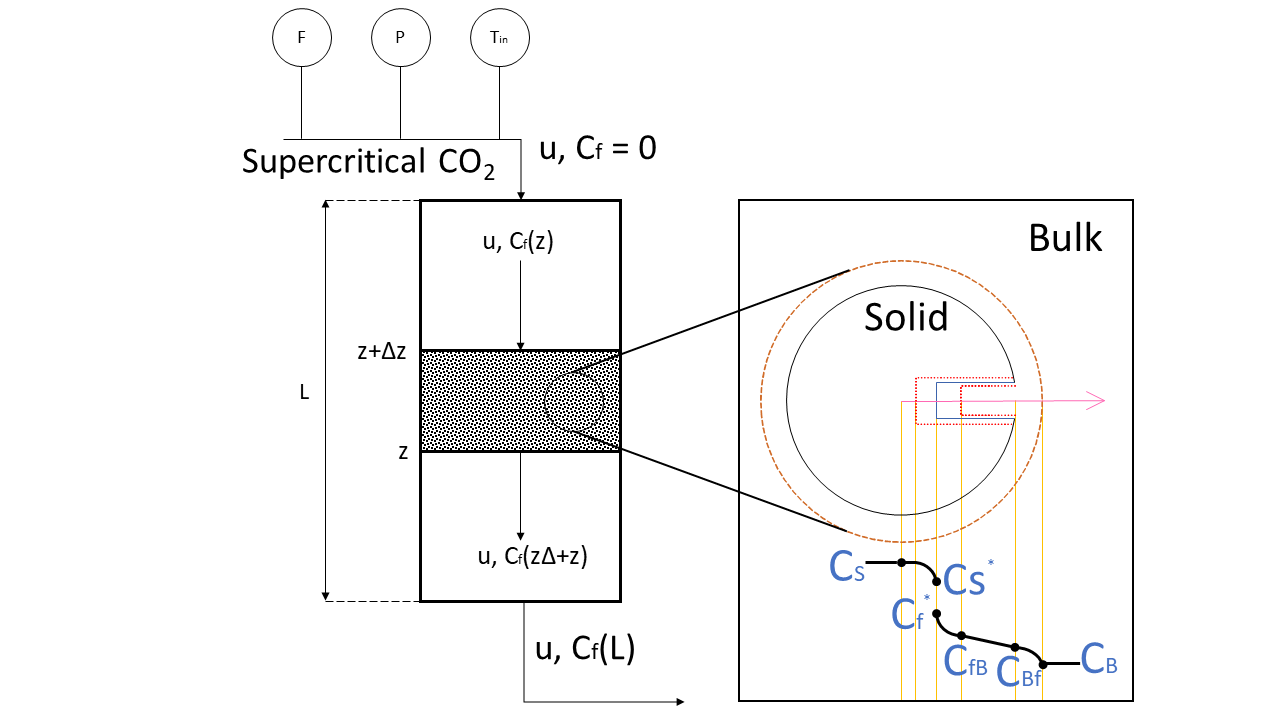
\includegraphics[trim  = 6cm 0cm 3cm 0cm,clip,width=\linewidth]{Figures/SFE_draft.png}
			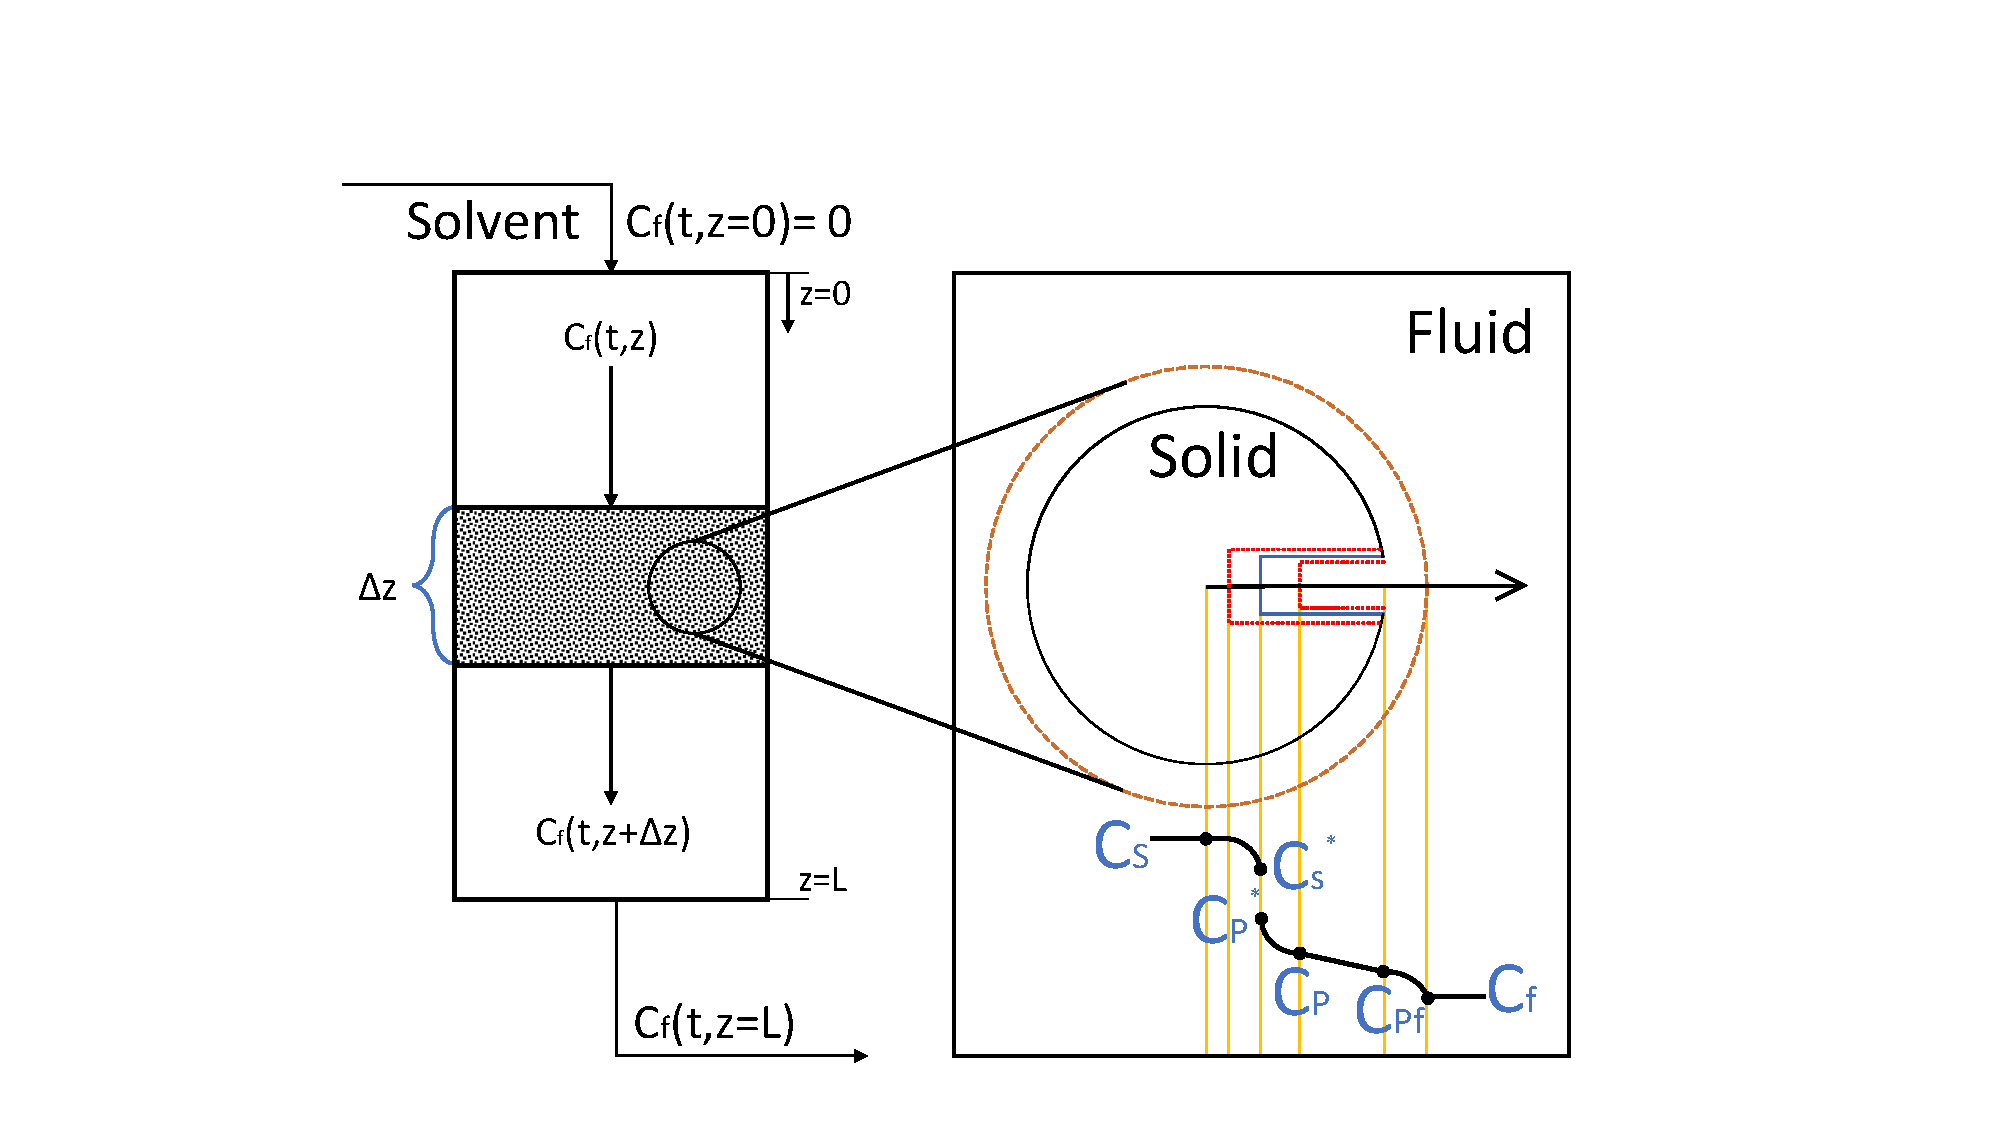
\includegraphics[trim = 5.8cm 1.1cm 6cm 3cm,clip,width=\columnwidth]{Figures/SFE_draft.pdf}	
			\caption{The extraction mechanism}
			\label{fig: SFE_Mechanism}
		\end{figure}
			
		\citet{Bulley1984} suggest a process where the driving force for extraction is given by the difference between concentration of the solute in the bulk, ${\color{blue}c_f}$, and in the centre of the pore, ${\color{blue}c_P^*}$. The concentration ${\color{blue}c_P^*}$ is in equilibrium with ${\color{blue}c_s}$ according to an equilibrium relationship. The rate of extraction is thus ${\color{blue}r_\text{e}}\left({\color{blue}c_f} - {\color{blue}c^*_P}({\color{blue}c_s})\right)$.  
			
		On the other hand, \citet{Reverchon1996} proposes a driving force given by the difference between ${\color{blue}c_s}$ and ${\color{blue}c_P^*}$. ${\color{blue}c_P^*}$ is determined by an equilibrium relationship with ${\color{blue}c_f}$ and the extraction rate is ${\color{blue}r_\text{e}}\left({\color{blue}c_s} - {\color{blue}c^*_P}({\color{blue}c_f})\right)$ or more precisely
			
			{\footnotesize
				\begin{equation} \label{Model_kinetic_basic}
					{\color{blue}r_e}(t,z) = \cfrac{{\color{orange}D_i}({\color{blue}T}(t,z), {\color{red}P}(t))}{{\color{magenta} \mu l^2} }\left({\color{blue}c_s}(t,z) - {\color{blue}c_P^*}(t,z) \right)
			\end{equation} }
			
		where ${\color{magenta}\mu}$ is sphericity, ${\color{magenta}l}$ a characteristic dimension of particles and can be defined as ${\color{magenta}l} = {\color{magenta}r}/3$, ${\color{magenta}r}$ is the mean particle radius, ${\color{magenta}\rho_s}$ is the solid density, ${\color{orange}D_i}({\color{blue}T}(t,z))$ corresponds to the overall diffusion coefficient and ${\color{blue}c_P^*}(t,z)$ is a concentration at the solid-fluid interface (which according to the internal resistance model is supposed to be at equilibrium with the fluid phase). 
			
		According to \citet{Bulley1984}, a linear equilibrium relationship (equation  \ref{Linear_equilibirum}) can be used to find an equilibrium concentration of the solute in the fluid phase ${\color{blue}c_f^*}(t,z)$ is based on concentration of the solute in the solid phase ${\color{blue}c_s}(t,z)$ 
			
			{\footnotesize
				\begin{align} \label{Linear_equilibirum}
					{\color{blue}c}(t,z) &= {\color{orange}k_p}({\color{blue}T}(t,z),{\color{red}P}(t)) \allowbreak {\color{blue}q^*}(t,z)
			\end{align} }
			
			The volumetric partition coefficient ${\color{orange}k_p}({\color{blue}T}(t,z),{\color{red}P}(t))$ behaves as an equilibrium constant between the solute concentration in one phase and the corresponding equilibrium concentration at the solid-fluid interphase. According to \citet{Spiro2007}, the term ${\color{orange}k_p}({\color{blue}T}(t,z),{\color{red}P}(t))$ can be expressed as the function of mass partition factor ${\color{orange}k_m}({\color{blue}T}(t,z))$.
			
			{\footnotesize
				\begin{align}
					{\color{orange}k_m}({\color{blue}T}(t,z)) = \cfrac{{\color{orange}k_p}({\color{blue}T}(t,z),{\color{red}P}(t)) {\color{magenta}\rho_s}}{{\color{orange}\rho}({\color{blue}T}(t,z),{\color{red}P}(t))}
			\end{align} }
			
			Equation \ref{Model_kinetic_no_sat} represents of the kinetic term according to \citet{Reverchon1996}
			
			{\footnotesize
				\begin{equation}
					\label{Model_kinetic_no_sat}
					{\color{blue}r_e}(t,z) = -\cfrac{{\color{orange}D_i}({\color{blue}T}(t,z), {\color{red}P}(t))}{{\color{magenta} \mu l^2} }\left({\color{blue}c_s}(t,z) - \cfrac{{\color{magenta}\rho_s}}{{\color{orange}k_m}({\color{blue}T}(t,z)){\color{orange}\rho_f}({\color{blue}T}(t,z),{\color{red}P}(t))}  {\color{blue}c_f}(t,z) \right)
			\end{equation} }

        %\subfile{Sections/Saturation}
			
		\subsubsection{Heat balance} \label{CH: heat_balance}
		
		\iffalse
		 {\color{red}
			The heat balance (equation \ref{Model_heat}) consists of the convective and diffusive terms. It follows the assumption of a pseudo-homogeneous phase, which properties are the mean between fluid and solid phases. We consider no heat loss through the wall, and there is no heat generation in the system. Therefore, the temperature of the extractor can be changed only by manipulating the temperature of the inlet stream %$T_{In}(t)$. 
			
			We assume that at a given section, where the cross-sectional area is $A$, the flow properties are uniform across that section. Hence, although the area of an extractor changes  as a function of a distance along an extractor (e.g. if a fixed fill an extractor partially), $z$, and therefore in reality the flow field is two-dimensional (the flow varies in the two-dimensional space), we make the assumption that the flow properties vary only with $z$; this is tantamount to assuming uniform properties across any given cross section. Such flow is defined as quasi-one-dimensional flow.
			
		}
		
		\sout{The heat balance equation (equation  \ref{Model_heat}) was developed, assuming the existence of a pseudo-homogeneous phase, which properties are the mean between fluid and solid phases (the amount of solute is considered small enough not to affect the overall heat balance). Equation \ref{Model_heat} contains the convection and the diffusion terms. It is considered that there is no heat loss through the wall, and there is no heat generation in the system. The temperature of the extractor can be changed only by increasing the temperature of the inlet stream. The pseudo-homogenous phase is assumed to flow only in the axial direction. The numerator of the factor in front of the convection term of the heat equation contains only the specific heat of the fluid ${\color{orange}C_p}({\color{blue}T}(t,z),{\color{red}P}(t))$ because the solid phase is stationary. Therefore, this factor can be understood as the fraction of the fluid's total heat through convection. On the other hand, the axial heat diffusion is calculated based on the definition of thermal diffusivity for the fluid, as explained in the appendix. }
			
		{\color{blue} The heat balance (equation \ref{Model_heat}), is based on \citet{Srinivasan2012}, and consists of convective and diffusive terms. It follows the assumption of a pseudo-homogeneous phase, which properties are the mean between fluid and solid phases. It is considered that there is no heat loss through the walls, and there is no heat generation in the system. The temperature of the extractor can be changed only by manipulating the temperature of the inlet stream ${\color{red}T_{Inlet}}(t)$.
			}
			
			{\footnotesize
				\begin{equation} \label{Model_heat}
					\begin{split}
						\cfrac{\partial {\color{blue}T}(t,z)}{\partial t} &= 
						\underbrace{ -\cfrac{{\color{red}F}(t) {\color{orange}C_p}({\color{blue}T}(t,z),{\color{red}P}(t))}{{\color{magenta}A} 	[(1-{\color{magenta}\epsilon}){\color{orange}\rho_f}({\color{blue}T}(t,z),{\color{red}P}(t)) {\color{orange}C_p} ({\color{blue}T}(t,z),{\color{red}P}(t)) + {\color{magenta} \epsilon \rho_s C_{ps} } ]} \cfrac{\partial {\color{blue}T}(t,z)}{\partial {\color{blue}z}}  }_{\text{Convection}} + \\
						& + \underbrace{ {\color{orange}D^T_e}({\color{blue}T}(t,z),{\color{red}P}(t)) \cfrac{\partial^2 {\color{blue}T}(t,z)}{\partial {\color{blue}z^2}} }_{\text{Diffusion}}
					\end{split}
			\end{equation} }
			
		where $ {\color{orange}D^M_e}({\color{blue}T}(t,z),{\color{red}P}(t),{\color{red}F}(t))$ is the axial mass diffusion coefficient, ${\color{orange}C_p}({\color{blue}T}(t,z),{\color{red}P}(t))$ is the fluid's specific heat, ${\color{magenta}C_{ps}}$ is the specific heat of the solid phase, ${\color{orange}D^T_e}({\color{blue}T}(t,z),{\color{red}P}(t),{\color{red}F}(t))$ is the axial heat diffusion coefficient. 

%		\todo[inline]{Draft of new heat equation starts here. TODO: \\ Check if the heat cpacity of solid phase needs to be added \\ Elaborate why pressure is know}
		\fi
		
			The heat equation was introduced in the previous chapter through equation \ref{EQ: CompressibleEuler_3} and in the appendix \ref{CH: Gouverning equations} 
			
			{\footnotesize
			\begin{align}
				&\cfrac{\partial \left( {\color{orange}\rho_f}({\color{blue}T}(t,z),{\color{red}P}(t)) {\color{blue}e}(t,z) A_f \right) }{\partial t} + \cfrac{\partial \left( {\color{orange}\rho_f}({\color{blue}T}(t,z),{\color{red}P}(t)) A_f v {\color{blue}e}(t,z) \right)}{\partial {\color{blue}z}} \nonumber \\
				&= -{\color{red}P}(t)\cfrac{\left( A_f v \right)}{\partial {\color{blue}z}} + \cfrac{\partial}{\partial {\color{blue}z}} \left( \cfrac{\partial {\color{blue}T}(t,z)}{\partial {\color{blue}z}} \right) 
			\end{align}
			}
		
			Following \citet{Elliott2011} or \citet{Gmehling2019}, a real gases internal energy definition can be obtained from the departure functions:

			{\footnotesize
				\begin{equation}
					d{\color{blue}e}(t,z)=C_vd{\color{blue}T}-\left[{\color{red}P}(t)-{\color{blue}T}(t,z)\left(\cfrac{\partial {\color{red}P}(t)}{\partial {\color{blue}T}(t,z)}\right)_{v_m}\right]dv_m
					\label{EQ: internal_energy_def}
				\end{equation} }
			
			where ${\color{blue}e}^{id}(t,z)$ is the internal energy of perfect gas.
			
			If a gas is consider to be perfectly caloric (${\color{blue}e}(t,z)=C_v {\color{blue}T}(t,z)$), then the energy equation can be written in form of temperature. The perfectly caloric gas can be seen as the special case of a real gas, where the second term of the equation \ref{EQ: internal_energy_def} goes to zero.
			
			For real gases it is complicated to write the heat balance in terms of temperature, but it be can used directly in the form of internal energy, as it is given by equation \ref{EQ: CompressibleEuler_3}. In such a case, the temperature (which is used as the input to some other functions) needs to be recover from the internal energy. A relation for the internal energy can be obtained from an equation of state. For Peng-Robinson, such a relation is given by equation \ref{EQ: internal_energy_PR} as presented by \citet{Elliott2011}.
			
%			{\footnotesize
%				\begin{equation}
%					e = C_vT + \cfrac{a\left(\alpha -T\cfrac{d \alpha}{dT}\right)}{2\sqrt{2}b} \ln \left[ \cfrac{1+b\left(1-\sqrt{2}\rho\right) }{1+b\left(1+\sqrt{2}\rho\right)} \right]
%					\label{EQ: internal_energy_PR}
%				\end{equation}
%			}
		
			{\footnotesize
				\begin{equation}
					\cfrac{{\color{blue}e}(t,z)-{\color{blue}e}^{id}(t,z)}{R{\color{blue}T}(t,z)} = - \cfrac{A}{B\sqrt{8}} \cfrac{\kappa \sqrt{T_r}}{\sqrt{\alpha}} \ln \left[ \cfrac{Z+\left( 1+\sqrt{2} \right)B}{Z+\left( 1+\sqrt{2} \right)B} \right]
					\label{EQ: internal_energy_PR}
				\end{equation}
			}
			
			To solve equation \ref{EQ: internal_energy_PR}, values of temperature, pressure and density needs to be know. If an equation of state is introduce, then only two out three variables needs to be know as the third one can be calculated, this can be represented as follow
			
			{\footnotesize
			\begin{equation}
				{\color{blue}e}(t,z)={\color{blue}e}({\color{blue}T}(t,z),{\color{red}P}(t),{\color{orange}\rho_f}({\color{blue}T}(t,z),{\color{red}P}(t)))=e( {\color{blue}T}(t,z),{\color{red}P}(t), \rho({\color{blue}T}(t,z),{\color{red}P}(t)) ) 
			\end{equation}
			}
		
			If the value of internal energy ${\color{blue}e}(t,z)$ is know from time evolution of the energy equation (\ref{EQ: CompressibleEuler_3}), and pressure is know from measurement, then the temperature can be reconstructed. A roootfinder can be used to find a value of temperature, which minimize the difference between value of internal energy coming from the time evolution and the output from equation \ref{EQ: internal_energy_PR}. Such a procedure allow to find local temperature along spatial direction ${\color{blue}z}$ and needs to be repeated every time-step.
			
			Another way to express the energy equation is to introduce enthalpy ${\color{blue}h}(t,z) = {\color{blue}e}(t,z) + {\color{red}P}(t) / \rho$. By introducing the definition of enthalpy, the energy equation becomes
			
			{\footnotesize
				\begin{align}
					&\cfrac{\partial \left({\color{orange}\rho_f}({\color{blue}T}(t,z),{\color{red}P}(t)) {\color{blue}h}(t,z) A_f\right)}{\partial t} - \cfrac{\partial \left({\color{red}P}(t) A_f\right)}{\partial t} \nonumber \\
					&+ \cfrac{\partial \left( {\color{orange}\rho_f}({\color{blue}T}(t,z),{\color{red}P}(t)) {\color{blue}h}(t,z) A_f v \right)}{\partial {\color{blue}z}} - \cfrac{\partial}{\partial {\color{blue}z}} \left( k \cfrac{\partial {\color{blue}T}(t,z)}{\partial {\color{blue}z}} \right)
				\end{align}
			}
		
			The main advantage of this formulation is the presence of term $\partial {\color{red}P}(t) / \partial t $, which allow to directly affect the system through the change of thermodynamic pressure (which is a control variable).\todo{ "For high pressures, the influence of the intermolecular forces on the enthalpy has to be taken into account, usually by applying a cubic equation of state. In most cases, these forces are attractive, so that additional energy is necessary to move the molecules away from each other, that is, to lower the density. If this energy is not added, the substance cools down when it is expanded" (\citet{Gmehling2019}). So, pressure reduction cause gas expansion and temperature drop.}
			If an equation of state is known, the temperature can to be recovered from the enthalpy. The enthalpy is related to the pressure and temperature through the following equation:
			
			{\footnotesize
				\begin{equation}
					{\color{blue}h}(t,z)=h({\color{blue}T}(t,z),{\color{red}P}(t),{\color{orange}\rho_f}({\color{blue}T}(t,z),{\color{red}P}(t)))=h( {\color{blue}T}(t,z),{\color{red}P}(t), \rho({\color{blue}T}(t,z),{\color{red}P}(t)) ) 
					\label{EQ:Enthalpy_root}
				\end{equation}
			}
		
			If the value of enthalpy is know from the time evolution and pressure can be measured, then the equation \ref{EQ:Enthalpy_root} can be solved for temperature to recover the temperature profile. By applying the departure functions to Peng-Robinson equation of state, the relation \ref{EQ:Enthalpy_root} can be expressed directly through equation \ref{EQ:Enthalpy_PR} as presented in \ref{CH:Enthalpy} or given by \citet{Gmehling2019}.
			
			{\footnotesize
				\begin{equation}
					{\color{blue}h}(t,z)-{\color{blue}h}(t,z)^{id}=R{\color{blue}T}(t,z) \left[T_{r}(Z-1)-2.078(1+\kappa ){\sqrt {\alpha }}\ln \left({\frac {Z+2.414B}{Z-0.414B}}\right)\right]
					\label{EQ:Enthalpy_PR}
				\end{equation}
			}
		
			The equation \ref{EQ:Enthalpy_PR} requires an reference sate, which in this case is assumed to be $T_{ref}=298.15~[K]$ and $P_{ref}=1.01325~[bar]$.
	
	
		\todo[inline]{Add short section about boundary conditions and comment on the used numerical methods}
  
		\subsubsection{Extraction yield} \label{CH: Yield} \todo{Give reference for measurement function}
			
		The efficiency of the process (the yield) is calculated according to equations \ref{Model_measurment_1} to \ref{Model_measurment_2}, which evaluate the mass of solute at the exit of the extraction unit and sums it. The integral form of the measurement equation can be transformed into the differential form, and augmented with model equations to be solved simultaneously.
			
		{\footnotesize
			\begin{align} 
				\label{Model_measurment_1}
%				y(t) \left[ kg \right] &= \int_{t_0}^{t_f} Q(t,z) \left[ \cfrac{m^3}{s} \right] c_f(t,z) \biggr\rvert_{z=L} \left[ \cfrac{kg}{m^3} \right] dt \left[ s \right] \\
				y(t) &= \int_{t_0}^{t_f} \cfrac{{\color{red}F}(t)}{{\color{orange}\rho_f}({\color{blue}T}(t,z),{\color{red}P}(t))} {\color{blue}c_f}(t,z) \biggr\rvert_{z=L} dt \\
%				\cfrac{dy}{dt} \left[ \cfrac{kg}{s} \right] &= Q(t,z) \left[ \cfrac{m^3}{s} \right] c_f(t,z) \biggr\rvert_{z=L} \left[ \cfrac{kg}{m^3} \right]  \\
				\cfrac{dy}{dt} &= \qquad \cfrac{{\color{red}F}(t)}{{\color{orange}\rho_f}({\color{blue}T}(t,z),{\color{red}P}(t))} {\color{blue}c_f}(t,z) \biggr\rvert_{z=L} 
                \label{Model_measurment_2}
		\end{align}	}
			
		\iffalse	
			
		\subsubsection{State-space representation} \label{CH: State_space}
		It is assumed that the solvent is free of solute at the entrance of the extractor and that all the solid particles have the same initial solute content ${\color{magenta}q_0}$. Moreover, it is considered that the initial temperature of the extractor in every place is equal to ${\color{magenta}T_0}$. Therefore, the initial conditions employed in the simulation are:
			
		{\footnotesize
			\begin{subequations}
				\begin{align*}
					{\color{blue}c}(t = 0, z) &= 0   \\
					{\color{blue}q}(t = 0, z) &= {\color{magenta}q_0} \\
					{\color{blue}T}(t = 0, z) &= {\color{magenta}T_0}
				\end{align*}
		\end{subequations} }
			
		The process model can be written in a general form:
			
		{\footnotesize
			\begin{align}
				\begin{bmatrix}
					\cfrac{\partial {\color{blue}c}(t,z)}{\partial t}\\
					\cfrac{\partial {\color{blue}q}(t,z)}{\partial t}\\
					\cfrac{\partial {\color{blue}T}(t,z)}{\partial t} 
				\end{bmatrix}
				& =
				\begin{bmatrix}
					{\color{blue}\phi_1} \left( {\color{blue}c}(t,z),{\color{blue}q}(t,z),{\color{blue}T}(t,z); {\color{magenta}\theta} \right)\\
					{\color{blue}\phi_2} \left( {\color{blue}c}(t,z),{\color{blue}q}(t,z),{\color{blue}T}(t,z); {\color{magenta}\theta} \right)\\
					{\color{blue}\phi_3} \left( {\color{blue}c}(t,z),{\color{blue}q}(t,z),{\color{blue}T}(t,z); {\color{magenta}\theta} \right)
				\end{bmatrix} = {\color{blue}\phi} \left( t,z; {\color{magenta}\theta} \right) = \cfrac{\partial {\color{blue}\chi}(t,z)}{\partial t}
		\end{align} }
			
		where ${\color{magenta}\theta}$ is a set of parameters present in the model, ${\color{blue}\phi}$ is a set of functions that correspond to state equations of the model, and ${\color{blue}\chi}$ is the state-space model.
		
		The method of lines is used to transform the process model equations into a set of ODEs denoted as ${\color{blue}G}({\color{blue}x}(t);{\color{magenta}p})$. The partial derivatives in $z$-direction are computed using a first-order and second-order finite difference approximation. The backward finite difference is used to approximate first-order derivative, while the central difference scheme is used to approximate second-order derivative. The length of the fixed bed is divided into $N_z$ equally distributed points in $z$-direction. Each function ${\color{blue}\phi_i}$ is transformed to a corresponding set of $N_z$ discretized equations denoted as ${\color{blue}G}_{i\times N_z+1}$ to ${\color{blue}G}_{(i+1)\times N_z}$, where $i$ corresponds to the process model equation. The state-space model ${\color{blue}\chi}(t,z)$ after the discretization is represented by $\dot{{\color{blue}x}}(t)$ (equation  \ref{discretization}).
			
			{\footnotesize
				\begin{align*} \label{discretization}
					\dot{{\color{blue}x}}(t) &= \cfrac{d {\color{blue}x}(t)}{d t} = 
					\begin{bmatrix}
						\cfrac{d {\color{blue}c_{f,1}}(t)}{d t} 	  \\
						\vdots					  \\
						\cfrac{d {\color{blue}c_{f,N_z}}(t)}{d t} \\
						\\ \hline \\
						\cfrac{d {\color{blue}c_{s,1}}(t)}{d t} 	  \\
						\vdots					  \\
						\cfrac{d {\color{blue}c_{s,N_z}}(t)}{d t} \\
						\\ \hline \\
						\cfrac{d {\color{blue}T_1}(t)}{d t} 	  \\
						\vdots 					  \\
						\cfrac{d {\color{blue}T_{N_z}}(t)}{d t}
					\end{bmatrix}
					=
					\underbrace{\begin{bmatrix}
							{\color{blue}G_1} \left( {\color{blue}x}(t),{\color{blue}q}(t),{\color{blue}T}(t); {\color{magenta}p} \right)\\ 
							\vdots\\ 
							{\color{blue}G_{N_z}} \left( {\color{blue}c}(t),{\color{blue}q}(t),{\color{blue}T}(t); {\color{magenta}p} \right)\\ 
							\\ \hline \\ \\
							{\color{blue}G_{N_z+1}} \left( {\color{blue}c}(t),{\color{blue}q}(t),{\color{blue}T}(t); {\color{magenta}p} \right)\\ 
							\vdots\\
							{\color{blue}G_{2N_z}} \left( {\color{blue}c}(t),{\color{blue}q}(t),{\color{blue}T}(t); {\color{magenta}p} \right)\\ 
							\\ \\ \hline \\ 
							{\color{blue}G_{2N_z+1}} \left( {\color{blue}c}(t),{\color{blue}q}(t),{\color{blue}T}(t); {\color{magenta}p} \right) \\
							\vdots\\
							{\color{blue}G_{3N_z}} \left( {\color{blue}c}(t),{\color{blue}q}(t),{\color{blue}T}(t); {\color{magenta}p} \right)
					\end{bmatrix}}_{{\color{blue}G} \left( {\color{blue}x}(t); {\color{magenta}p} \right)} 
			\end{align*} }
			
			where ${\color{blue}x} \in \mathbb{R}^{N_x = 3N_z} $ and ${\color{magenta}p} \in \mathbb{R}^{N_p =  N_{\theta} + N_u } $, $N_{\theta}$ is the number of model parameters, $N_{u}$ is the number of control variables.
			
			{\color{blue} In a state-space sense, the state variables of the system are the local concentrations of solute in the fluid and solid phases ($c(t,z)$ and $q(t,z)$, respectively), and the local temperature of the pseudo-homogeneous phase ($T(t,z)$). The controllable input variables are the mass flow-rate and temperature of the solvent in the feed ($F_\text{in}(t) = {\color{red}P}(t)$ and $T_\text{in}(t) = T(t,z=0)$, respectively) and the pressure in the extractor ($P(t,z) ={\color{red}P}(t)$). {\color{red}We also assume that extraction yield can be modelled as a function of a known initial mass of solute in the solid phase and it can be measured after the separator ($Y(t)$).} The system is controllable by manipulating the flow-rate and temperature of CO2 in the feed, and the pressure in the extractor. }
			
			\fi
			
\end{document}